\documentclass{article}
\usepackage{amsthm}
\usepackage[dvipsnames]{xcolor}
\usepackage{avant}
\usepackage{fancyhdr}
\usepackage{tikz}
\usetikzlibrary{shapes, positioning}
\usepackage{hyperref}
\usepackage[bottom]{footmisc}

\renewcommand{\familydefault}{\sfdefault}   % cambio font
\theoremstyle{definition}
\newtheorem*{definition}{Definizione}
\renewcommand{\contentsname}{Contenuti}

\pagestyle{fancy}
\fancyfoot[L]{Ingegneria del Software}
\fancyfoot[C]{\thepage}
\fancyfoot[R]{Angelo Passarelli}

\setcounter{section}{-1}

\title{Ingegneria del Software}
\author{Angelo Passarelli}
\date{\today}

\begin{document}    
    \maketitle
    \begin{center}
        \includegraphics[scale=0.15]{img/Stemma_unipi.png}
    \end{center}
    \vspace{1cm}
    \begin{center}
        Appunti basati sulle lezioni e dispense della professoressa Laura Semini \footnote{\url{http://didawiki.cli.di.unipi.it/doku.php/informatica/is-a/start}}
    \end{center}
    \pagebreak
    \tableofcontents
    \pagebreak

    \begin{sloppypar}
        
        \section{Introduzione}
\subsection*{Fasi del progetto}
\begin{center}
    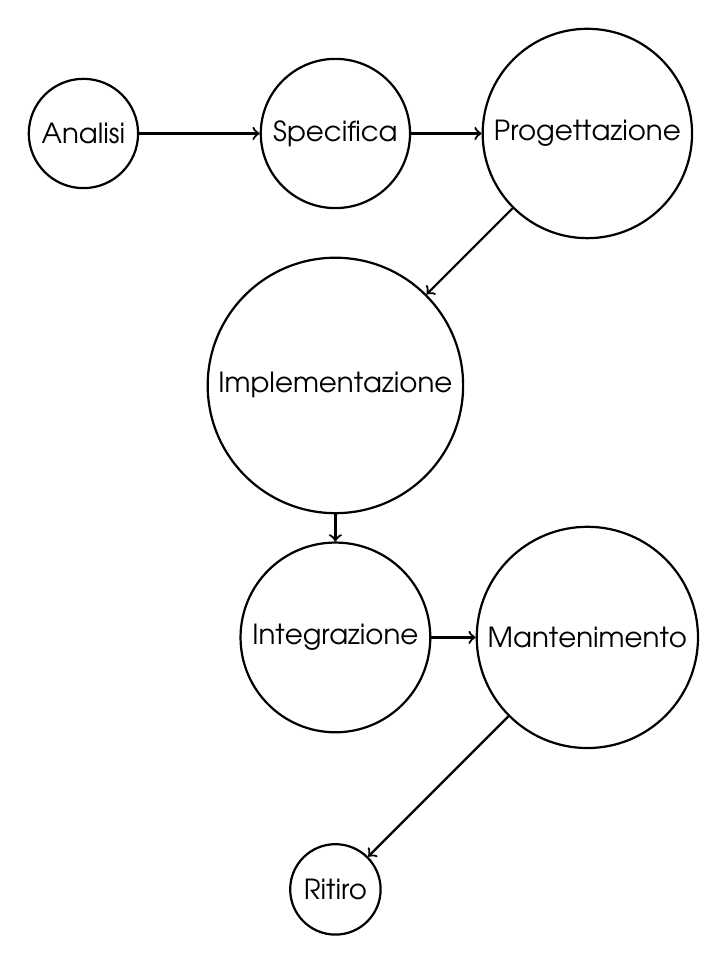
\begin{tikzpicture}[node distance={32mm}, thick, main/.style = {draw, circle}]
        \node[main] (1) {Analisi};
        \node[main] (2) [right of=1] {Specifica};
        \node[main] (3) [right of=2] {Progettazione}; 
        \node[main] (4) [below of=2] {Implementazione};
        \node[main] (5) [below of=4] {Integrazione}; 
        \node[main] (6) [right of=5] {Mantenimento};
        \node[main] (7) [below of=5] {Ritiro};
        \draw[->] (1) -- (2);
        \draw[->] (2) -- (3);
        \draw[->] (3) -- (4);
        \draw[->] (4) -- (5);
        \draw[->] (5) -- (6);
        \draw[->] (6) -- (7);
    \end{tikzpicture}
\end{center}
\subsection*{Specificità del Software}
    \begin{enumerate}
        \item \textbf{\textcolor{cyan}{Fault toulerance}}: capacità del software di essere tollerante ai guasti.
        \item \textbf{\textcolor{cyan}{Difetto latente}}: difetto nascosto che si trova difficilmente in fase di testing; e anche nel caso comparisse è quasi impossibile da ritrovare.
        \item \textbf{\textcolor{cyan}{Robustezza}}: capacità di funzionare anche con input non previsti e/o non testati.
        \item Il software non presenta \textcolor{cyan}{costi materiali} e nemmeno \textcolor{cyan}{costi marginali}, ovvero il costo di un'unità del prodotto.
        \item Infine il software non si consuma nel tempo, ma potrebbe diventare \textcolor{cyan}{obsoleto}.
    \end{enumerate}
\subsection*{La Manutenzione}
    \paragraph{Costi} 
    La fase di manutenzione è quella che richiede costi più alti. 
    Per evitare uno spreco durante questa fase è necessario studiare bene l'analisi dei requisiti, in quanto un errore in questa fase
    si propagherà in modo esponenziale, in termini di costi, nelle fasi successive.
    \break
    \break
    La manutenzione si divide in:
    \begin{itemize}
        \item \textbf{\textcolor{cyan}{Manutenzione Correttiva}}: rimuove gli errori, lasciando invariata la specifica.
        \item \textbf{\textcolor{cyan}{Manutenzione Migliorativa}}: consiste nel cambiare quella che è la specifica, e a sua volta può dividersi in:
            \begin{itemize}
                \item \textcolor{cyan}{Perfettiva}: modifiche per migliorare e/o introdurre nuove funzionalità.
                \item \textcolor{cyan}{Adattiva}: modifiche indotta da cambiamenti esterni, come leggi o modifiche all'hardware o al sistema operativo.
            \end{itemize}
    \end{itemize}
    \subsection*{Stakeholders}
        \begin{itemize}
            \item \textcolor{cyan}{Fornitore}: colui che sviluppa il software.
            \item \textcolor{cyan}{Committente}: chi lo richiede e paga.
            \item \textcolor{cyan}{Utente}: chi lo usa.
        \end{itemize}
        \section{Modelli di Ciclo di Vita}

\begin{definition}[Processo Software]
    Con processo software si indica il percorso da seguire per sviluppare un prodotto o più nello specifico un software.
    Fanno parte del processo sia gli strumenti e le tecniche per lo sviluppo che i professionisti coinvolti.
\end{definition}

\subsection{Modelli Sequenziali}

\subsubsection{Build-and-Fix}

Il prodotto è sviluppato senza alcuna fase di progettazione preliminare, lo sviluppatore scrive il software
e poi lo modifica ogni volta che non soffisfa il committente.

\paragraph{\textcolor{red}{Contro}}

Diventa improponibile per progetti grandi e la manutenzione diventa difficile senza documentazione nè specifica.

\subsubsection{Modello a Cascata}

Questo modello è stato il primo a distingure il processo software in più fasi, evidenziando l'importanza della progettazione e dell'analisi.

Viene chiamato anche modello \emph{\textcolor{cyan}{document driven}} dato che ogni fase produce un documento, e per passare alla successiva
occorre aver approvato il documento della fase precedente.

\paragraph{\textcolor{red}{Contro}} Troppo pesante da seguire, inoltre non si può tornare indietro, e mancando
l'interazione con il cliente, se non è soddisfatto, và tutto ripetuto dall'inizio.

\subsubsection{Modello a V}

\begin{center}
    \begin{figure}[h]
            \includegraphics[scale=0.5]{img/V-model.JPG}
        \caption{Le frecce blu rappresentano il \emph{tempo}, mentre quelle tratteggiate le \emph{dipendenze}}
    \end{figure}
\end{center}

Questo modello evidenzia come sia possibile progettare i \textcolor{cyan}{test}
durante le fasi di sviluppo (quelle a sinistra, prima della fase di \emph{coding}). Mentre sulla destra
sono presenti i test veri e propri che devono verificare e convalidare l'attività in corrispondenza sulla sinistra.

\paragraph{\textcolor{ForestGreen}{Standard SQA}}
Questo modello è uno degli standard \emph{SQA} (Software Quality Assurance), usato
per descrivere le attività di test durante il processo di sviluppo.

\subsection{Modelli Iterativi}

\subsubsection{Rapid Prototyping}

L'obbiettivo è quello di costruire rapidamente un prototipo del software per permettere al committente di sperimentarlo.

Questo modello diventa utile quando i requisiti non sono chiari, quindi ogni prototipo aiuterà il cliente a descriverli meglio.

\begin{center}
    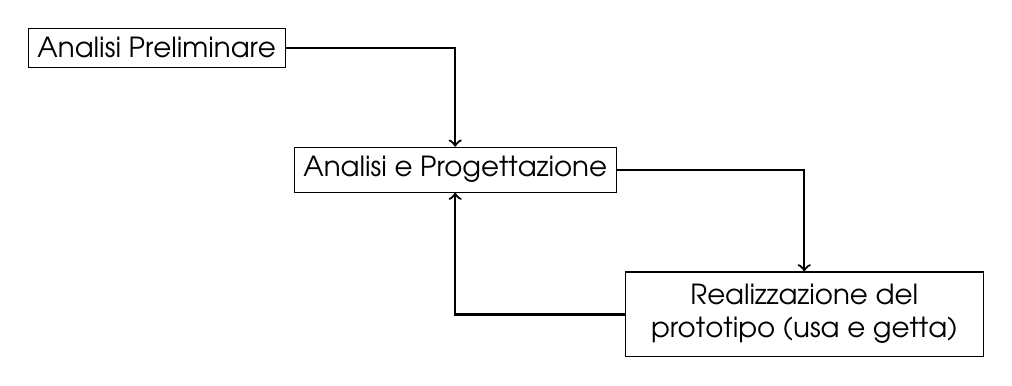
\begin{tikzpicture}[main/.style={rectangle, draw}]
        \node[main] (1) {Analisi Preliminare};
        \node[main] (2) [below right=1cm and 0.1cm of 1] {Analisi e Progettazione};
        \node[main] (3) [below right=1cm and 0.1cm of 2] {\begin{tabular}{c}Realizzazione del \\ prototipo (usa e getta)\end{tabular}};
        \draw[thick, ->] (1) -| (2);
        \draw[thick, ->] (2) -| (3);
        \draw[thick, ->] (3) -| (2);
    \end{tikzpicture}
\end{center}

\subsubsection{Modello Incrementale}

Il software viene costruito in modo iterativo, aggiungendo di volta in volta nuove funzionalità.

I requisiti e la progettazione vengono definiti inizialmente, per questo è possibile applicarlo solo in caso di requisiti stabili.

\paragraph{\textcolor{red}{Contro}}
Se non viene realizzata una buona progettazione, questo modello sfocia in un \emph{Build-and-Fix}.

\begin{center}
    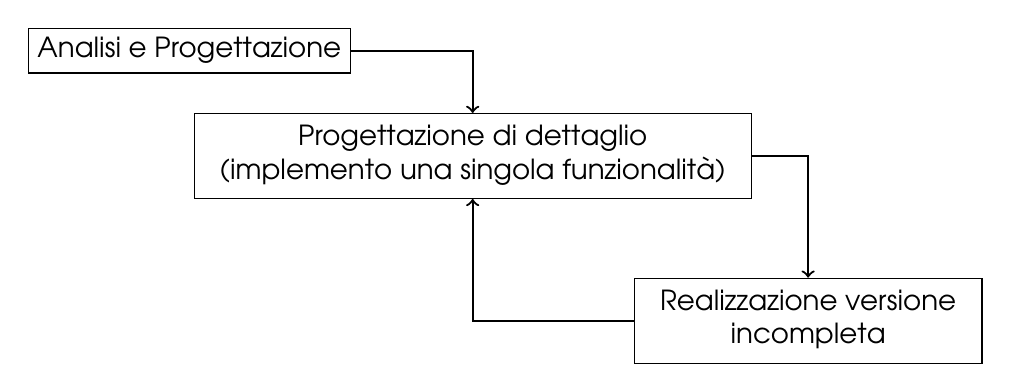
\begin{tikzpicture}[main/.style={rectangle, draw}]
        \node[main] (1) {Analisi e Progettazione};
        \node[main] (2) [below right=0.5cm and -2cm of 1] {\begin{tabular}{c} Progettazione di dettaglio \\ (implemento una singola funzionalità) \end{tabular}};
        \node[main] (3) [below right=1cm and -1.5cm of 2] {\begin{tabular}{c} Realizzazione versione \\ incompleta \end{tabular}};
        \draw[thick, ->] (1) -| (2);
        \draw[thick, ->] (2) -| (3);
        \draw[thick, ->] (3) -| (2);
    \end{tikzpicture}
\end{center}

\newpage

\subsubsection{Modello a Spirale}

In questo caso ogni iterazione è formata da 4 fasi che corrispondono ai quadranti del piano:
\begin{enumerate}
    \item \emph{Quadrante in alto a sinistra}: definizione degli obiettivi e dei vincoli.
    \item \emph{Quadrante in alto a destra}: analisi e risoluzione dei rischi.
    \item \emph{Quadrante in basso a destra}: sviluppo e verifica del prossimo livello.
    \item \emph{Quadrante in basso a sinistra}: pianificazione della fase successiva.
\end{enumerate}

Questo modello viene anche chiamato \emph{\textcolor{cyan}{risk driven}} in quanto è incentrato principalmente sull'analisi
dei rischi. Inoltre si ispira profondamente al metodo iterazivo \emph{\textcolor{cyan}{plan-do-check-act cycle}} \footnote{\url{https://it.wikipedia.org/wiki/Ciclo_di_Deming}}

\begin{figure}[h]
    \begin{center}
        \includegraphics[scale=0.4]{img/modellospirale.png}
    \end{center}
\end{figure}

\subsection{Unified Process}

In questo modello vengono distinte quattro fasi chiamate \emph{\textcolor{cyan}{Inception}}, \emph{\textcolor{cyan}{Elaboration}}, \emph{\textcolor{cyan}{Construction}}
e \emph{\textcolor{cyan}{Transition}}. Ogni fase può presentare un numero variabile di iterazioni anche in base alla dimensione
del progetto.

Questo modello viene definito \textcolor{cyan}{iterativo incrementale}, \emph{incrementale} perchè
alla fine di ogni iterazione si ottiene un rilascio del sistema con funzionalità in più o migliorate
rispetto al rilascio precedente.

Inoltre viene data molta importanza all'architettura del sistema, infatti già dalle prime fasi ci si
concentra soprattutto sull'architettura anche se a livello molto superficiale, lasciando i dettagli alle fasi successive. In questo
modo è molto facile avere una visione generale del sistema che sarà facilmente modellabile sulla variazione dei requisiti. Per
questo, piuttosto che dai requisiti, ci si fà guidare principalmente dai \emph{casi d'uso} e dall'\emph{analisi dei rischi}.

\begin{figure}[h]
    \begin{center}
        \includegraphics[scale=0.8]{img/unified_process.png}
    \end{center}
\end{figure}

\subsection{Processi Agili}

\begin{definition}[Metodo Agile]
    Con \textcolor{cyan}{metodo agile} si intende un metodo per lo sviluppo del software
    che si basa principalmente sul coinvolgimento del committente.
    Questa metodologia si riferisce ai principi del \emph{\textcolor{cyan}{Manifesto di Snowbird}} del 2001.
\end{definition}

I concetti chiave di questi processi sono:

\begin{itemize}
    \item \textcolor{cyan}{Continuous Integration}: rendere il più automatico possibile la consegna e l'integrazione dei singoli moduli.
    \item \textcolor{cyan}{Continuous Delivery}: rilascio frequente e supportato delle nuovi versioni del software.
    \item \textcolor{cyan}{DevOps}: \emph{Development} e \emph{Operations}, ovvero maggiore collaborazione tra sviluppatori e responsabili della
        manutenzione, della sicurezza e dell'infrastruttura dell'azienda.
\end{itemize}

\subsubsection{Il Manifesto di Snowbird}

Il \emph{Manifesto di Snowbird} si fonda su quattro punti fondamentali:

\begin{enumerate}
    \item \textcolor{cyan}{Comunicazione}: la comunicazione fra tutti gli attori del progetto è centrale, soprattutto le interazioni e
        la collaborazione con i clienti.
    \item \textcolor{cyan}{Semplicità}: si mantiene il codice sorgente il più semplice possibile, ma comunque avanzato tecnicamente,
        in questo modo si riduce la documentazione al minimo indispensabile.
    \item \textcolor{cyan}{Feedback}: sin dal primo giorno di sviluppo il codice viene testato, in modo da poter rilasciare versioni ad intervalli molto frequenti.
    \item \textcolor{cyan}{Coraggio}: dare in uso il sistema il prima possibile ed implementare i cambiamenti richiesti man mano.
\end{enumerate}

Di seguito sono riportati due modelli che si basano sui \emph{processi agili}.

\subsubsection{eXtreme Programming}

Si basa su un insieme di consuetudini:

\begin{itemize}
    \item \emph{Pianificazione flessibile}: è basata su un insieme di scenari proposti dagli utenti e i programmatori vengono coinvolti direttamente.
    \item \emph{Rilasci frequenti}: più o meno ogni 2-4 settimane, e alla fine si ricomincia con una nuova pianificazione.
    \item \emph{Progetti semplici}: comprensibili a tutti.
    \item \emph{Testing}: test basati sui singoli scenari e con supporto automatico.
    \item \emph{Test Driven Development}: i casi di test vengono definiti prima della scrittura del codice.
    \item \emph{Cliente sempre a disposizione}
    \item \emph{Programmazione a coppie}: viene usato un solo terminale, una persona svolge il ruolo di \emph{\textcolor{cyan}{driver}}
        che scrive il codice, mentre un'altra fà il \emph{\textcolor{cyan}{navigatore}}, ovvero controlla il lavoro del \emph{driver} attivamente.
    \item \emph{No al lavoro straordinario}
    \item \emph{Collettivizzazione del codice}: accesso libero e continua integrazione.
    \item \emph{Code Refactoring}: modificare il codice senza cambiare il suo comportamento e commentarlo il più possibile.
    \item \emph{Daily Stand Up Meeting}
\end{itemize}

\subsubsection{SCRUM}

\begin{definition}[SCRUM]
    Con \emph{\textcolor{cyan}{SCRUM}} si intende un processo \emph{iterativo} ed \emph{incrementale}, dove alla fine
    di ogni iterazione vengono rilasciate un insieme di funzionalità potenzialmente rilasciabili.
\end{definition}

Il processo è diviso in tre fasi:

\begin{enumerate}
    \item \textbf{\textcolor{cyan}{Pre-game phase}}: 
        \begin{enumerate}
            \item \textcolor{cyan}{Planning sub-phase}: viene creata una \emph{\textcolor{cyan}{Product Backlog List}}
                che contiene tutti i requisiti conosciuti.
            \item \textcolor{cyan}{Architecture sub-phase}: viene già pianificato il design di alto livello e l'architettura del sistema.
        \end{enumerate}
    \item \textbf{\textcolor{cyan}{Development phase}}: in questa fase il sistema viene sviluppato attraverso una serie di \emph{\textcolor{cyan}{Sprint}},
        ovvero cicli iterativi nei quali vengono sviluppate o migliorate una serie di funzionalità, e ogni sprint può durare circa 1-4 settimane. Lo \emph{Sprint} ovviamente
        include le classiche fasi di sviluppo del software.
    \item \textbf{\textcolor{cyan}{Post-game phase}}: il prodotto viene preparato per il rilascio, ovvero si prepara l'\emph{integrazione},
        i \emph{test}, la \emph{documentazione} per l'utente e la preparazione del materiale di \emph{marketing}.
\end{enumerate}

I ruoli principali durante l'esecuzione di un processo \emph{SCRUM} sono tre:

\begin{itemize}
    \item \textbf{\textcolor{cyan}{Product Owner}}: ci si riferisce a quella persona responsabile di accettare o rifiutare i risultati di un lavoro e di poter terminare uno \emph{Sprint}, inoltre
        fà da raccordo fra tutti soggetti interessati nel progetto.
    \item \textbf{\textcolor{cyan}{Membri del Team}}: i membri decidono cosa fare in ogni \emph{Sprint}, ogni team è indipendente e i membri non fanno capo ad alcun project manager.
        Ogni membro ha diverse specializzazioni (\emph{cross-functional}), in modo tale da non avere persone con troppo carico di lavoro e ognuno si occupa di un singolo lavoro alla volta.
    \item \textbf{\textcolor{cyan}{Scrum Master}}: non ha alcuna autorità sul team, ma si occupa di supportarlo e motivarlo, garantendo anche le condizioni ambientali per lavorare al meglio.
\end{itemize}

\paragraph{Kanban Board} Questa lavagna permette di gestire al meglio il flusso del lavoro. Come mostrato in figura è presente
un \emph{\textcolor{cyan}{Work In Progress Limit}} che definisce un limite alla quantità di post-it che possono essere presenti in
ogni colonna. Questo limite permette di completare più velocemente i singoli lavori, in modo tale di dare qualcosa al cliente il prima possibile e di
individuare facilmente i \textcolor{cyan}{colli di bottiglia} che possono rallentare gli altri lavori.
Inoltre permette di ridurre il \emph{\textcolor{cyan}{task switching}}, ovvero il lavoro su più task contemporaneamente.

\begin{figure}[h]
    \begin{center}
        \includegraphics[scale=0.5]{img/kanboard.png}
    \end{center}
\end{figure}

Gli eventi che fanno parte di uno \emph{Sprint} sono i seguenti:
\begin{enumerate}
    \item \textcolor{cyan}{Sprint planning}: il \emph{product owner} gestisce l'evento di pianificazione dello \emph{Sprint}.
    \item \textcolor{cyan}{Daily meeting}: i membri del team e gli SCRUM master si ritrovano davanti la \emph{kanban} e discutono delle
        difficultà che hanno riscontrato.
    \item \textcolor{cyan}{Review}: alla fine di di una modifica concreta al software, questo viene ispezionato in collaborazione con gli utenti per ottenere un feedback
        e per discutere su cambiamenti o nuove idee.
    \item \textcolor{cyan}{Retrospettiva}: questa fase permette di riflettere, studiare e adattarsi per lo \emph{Sprint} successivo.
\end{enumerate}
        \section{Analisi dei Requisiti}

\begin{definition}[Analisi dei Requisiti]
    Si intende il processo di studio e analisi delle esigenze del committente e dell'utente per
    giungere alla produzione di un documento che definisce il \emph{dominio} del problema e i \emph{requisiti} del software.
    In alcuni casi si definiscono anche i \emph{casi di test} e il \emph{manuale utente}.
\end{definition}

Prima di passare alla fase vera e propria di \emph{analisi dei requisiti}
occorre seguire una fase preliminare per stabilire la realizzabilità
del progetto software.

\subsection{Studio di Fattibilità}

Si basa principalmente sulla descrizione del software e delle necessità
dell'utente. In seguito vengono svolte due analisi:

\begin{itemize}
    \item \textcolor{cyan}{Analisi di Mercato}: si fà un confronto con il mercato attuale e si stimano i costi di
        produzione e quanto l'investimento può essere remunerativo.
    \item \textcolor{cyan}{Analisi Tecnica}: si studiano tutti gli strumenti per la realizzazione del progetto,
        come i software, le architetture, gli hardware e gli algoritmi. Inoltre si studia come deve essere fatta la prototipazione
        del software e la futura ricerca. 
\end{itemize}

\subsection{Dominio}

Il \textbf{\textcolor{cyan}{dominio}} è il contesto in cui il software opera. Per definirlo occorre costruire
un \textcolor{cyan}{glossario}, ovvero una collezione di definizioni di termini rilevanti in quel dominio specifico e
che può essere riusato in progetti successivi nello stesso dominio. Inoltre occorre definire un \textcolor{cyan}{modello statico},
quindi come interagiscono fra loro gli elementi del dominio staticamente, e un \textcolor{cyan}{modello dinamico}, ovvero come si comporta il dominio
in base all'avvenire di un determinato evento che può coinvolgere gli utenti. Questi due modelli possono essere descritti sia 
tramite l'uso del linguaggio UML \footnote{\url{https://it.wikipedia.org/wiki/Unified_Modeling_Language}}, sia usando la semplice descrizione testuale.

\subsection{Requisiti}

\begin{definition}[Requisito]
    Il requisito è una proprietà che deve essere garantita dal sistema per soddisfare
    una qualsiasi necessità dell'utente.
\end{definition}

I requisiti possono dividersi in due categorie:
\begin{itemize}
    \item \textbf{\textcolor{cyan}{Requisiti funzionali}}: quelli che descrivono le funzionalità e il comportamento del software.
    \item \textbf{\textcolor{cyan}{Requisiti non funzionali}}: descrivono le proprietà del software o del processo di sviluppo. Ad esemprio le caratteristiche di
        efficienza e affidabilità, l'interfaccia, il linguaggio di programmazione e l'ambiente di sviluppo scelti, i vincoli legislativi e i requisiti hardware o di rete.
\end{itemize}

I requisiti possono essere descritti mediante l'uso di diversi linguaggi, formali o meno. In questo caso si vede
la descrizione dei requisiti mediante la produzione di un documento scritto in linguaggio naturale.

\subsection{Documento dei Requisiti}

Questo documento è un contratto tra lo sviluppatore e il committente, che elenca i requisti e i vincoli che il software deve soddisfare, e specifica
anche una \emph{deadline} per la consegna del progetto.

\subsection{Fasi dell'Analisi dei Requisiti}

L'\emph{analisi dei requisiti} viene svolta in cinque passi:
\begin{enumerate}
    \item \textbf{\textcolor{cyan}{Acquisizione}}
    \item \textbf{\textcolor{cyan}{Elaborazione}}
    \item \textbf{\textcolor{cyan}{Convalida}}
    \item \textbf{\textcolor{cyan}{Negozazione}}
    \item \textbf{\textcolor{cyan}{Gestione}}
\end{enumerate}

\subsubsection{Acquisizione}

Il team di analisti incontra i membri dell'organizzazione del committente e si procede con
la raccolta dei requisiti che può avvenire tramite: semplici interviste, questionari, costruzione di
prototipi (anche su carta), studio di documenti o l'osservazione di possibili utenti mentre lavorano.

\subsubsection{Elaborazione}

Viene scritta la prima bozza del \emph{documento dei requisti}, dove quest'ultimi vengono trattati in modo
più approfondito. La struttura del documento deve essere la seguente:

\begin{center}
    \begin{tabular}{||c||}
        \hline
        \emph{Introduzione} \\
        \hline
        \emph{Glossario} \\
        \hline
        \emph{Definizione dei Requisiti Funzionali} \\
        \hline
        \emph{Definizione dei Requisiti Non Funzionali} \\
        \hline
        \emph{Architettura}: la strutturazione del software in sottosistemi. \\
        \hline
        \emph{Specifica dettagliata dei Requisiti Funzionali} \\
        \hline
        \emph{Modelli astratti}: descrivere il sistema in base \\ a ciascun punto di vista. \\
        \hline
        \emph{Evoluzione del sistema}: successivi cambiamenti. \\
        \hline
        \emph{Appendici}: descrizione della piattaforma hardware, database, \\ manuale utente e i piani di test. \\
        \hline
        \emph{Indici}: costruire un lemmario, quindi una lista di termini \\ che puntano ai requisiti che li usano. \\
        \hline
    \end{tabular}
\end{center}

\paragraph{Nota Bene} Nella descrizione dei requisiti occorre sempre usare la forma assertiva.
Esempio:
\begin{center}
    \emph{Il $<$sistema$>$ deve $<$funzionalità$>$/$<$proprietà$>$}
\end{center}

\subsubsection{Convalida}

Nella fase di convalida occorre revisionare il documento per far sì che vengano
evitati i seguenti difetti:

\begin{itemize}
    \item \textcolor{cyan}{Omissioni}: requisiti mancanti.
    \item \textcolor{cyan}{Inconsistenze}: contraddizione tra i requisiti o tra un requisito e il contesto.
    \item \textcolor{cyan}{Ambiguità}: vaghezze o requisiti che possono avere più significati. Le ambiguità all'interno del linguaggio naturale
        possono essere portate da \textcolor{MidnightBlue}{quantificatori}, \textcolor{MidnightBlue}{disgiunzioni}
        oppure possono presentarsi ambiguità di \textcolor{MidnightBlue}{coordinazione} (nel caso si usano sia la \emph{o} che la \emph{e} nella stessa frase) oppure 
        \textcolor{MidnightBlue}{referenziale} nell'uso non chiaro di pronomi.
        Inoltre occorre sempre evitare \textcolor{MidnightBlue}{verbi deboli}, \textcolor{MidnightBlue}{forme passive}, ovvero verbi senza un soggetto esplicito ed anche \textcolor{MidnightBlue}{negazione}
        e \textcolor{MidnightBlue}{doppie negazioni}.
    \item \textcolor{cyan}{Sinonimi} e \textcolor{cyan}{Omonimi}: termini diversi con lo stesso significato e termini uguali con significato diverso.
    \item \textcolor{cyan}{Presenza di dettagli tecnici}
    \item \textcolor{cyan}{Ridondanza}: può esserci, ma solo tra sezioni diverse del documento.
\end{itemize}

Le principali tecniche di convalida dei requisiti sono:
\begin{itemize}
    \item \textcolor{cyan}{Deskcheck}
        \begin{itemize}
            \item \textcolor{cyan}{Walkthrough}: ovvero il documento viene analizzato per intero sequenzialmente.
            \item \textcolor{cyan}{Ispezione}: la lettura del documento è strutturata, utilizzando per esempio la tecnica del
                lemmario.
        \end{itemize}
    \item Uso di \textcolor{cyan}{strumenti di analisi} del linguaggio naturale.
    \item Uso di \textcolor{cyan}{prototipi}.
\end{itemize}

Una volta trovati i difetti, è importante ricordarsi che vanno sempre risolti con
il committente.

\subsubsection{Negoziazione}

In questa fase vengono assegnate delle priorità ai requisiti in base alle
\textcolor{cyan}{esigenze del committente} e ai \textcolor{cyan}{costi} e \textcolor{cyan}{tempi} di
produzione.

Questa fase è importante per decidere se alcuni requisiti possono essere \textcolor{cyan}{cancellati} oppure
\textcolor{cyan}{sviluppati} successivamente.

\paragraph{MoSCoW} Questa è una tecnica per dare priorità ai requisiti, i quali vengono divisi in quattro classi:
\begin{itemize}
    \item \textcolor{cyan}{Must have}: requisiti irrinunciabili per il cliente.
    \item \textcolor{cyan}{Should have}: non necessari ma utili.
    \item \textcolor{cyan}{Could have}: non molto utili, da realizzare solo se c'è tempo.
    \item \textcolor{cyan}{Want to have}: da sviluppare in successive versioni.
\end{itemize}

\subsubsection{Gestione}

Questa fase si occupa di tre aspetti principali:
\begin{itemize}
    \item \textcolor{cyan}{Identificazione}: ad ogni requisito viene assegnato un identificatore univoco.
    \item \textcolor{cyan}{Attributi}: ad ogni requisito vengono assegnati attributi relativi allo \textcolor{MidnightBlue}{stato},
        \textcolor{MidnightBlue}{priorità}, \textcolor{MidnightBlue}{sforzo} in termini di giorni e/o personale da impiegare, \textcolor{MidnightBlue}{rischio},
        e la \textcolor{MidnightBlue}{versione destinazione} per quanto riguarda lo sviluppo incrementale. 
    \item \textcolor{cyan}{Tracciabilità}: ovvero la capacità di descrivere e seguire la vita di un requisito. Viene costruita una mappa tra i requisiti
        e le \textcolor{MidnightBlue}{componenti del sistema}, il \textcolor{MidnightBlue}{codice} ed i \textcolor{MidnightBlue}{test}.
\end{itemize}

\paragraph{Contratto} Il \emph{documento dei requisiti} precede la stipula del contratto.

\subsection{Casi d'uso}

I \textbf{\textcolor{cyan}{casi d'uso}} sono un altro modo per acquisire i requisiti, valutando le interazioni degli utenti col sistema
e indicando al committente i risultati attesi. I casi d'uso oltre ad includere la sequenza corretta di eventi attesi devono anche presentare i comportamenti inattesi,
ovvero le \textcolor{cyan}{eccezioni}.

\subsection{User Stories}

Sono un'altra tecnica di raccolta dei requisiti utilizzata principalmente nei \emph{\textcolor{cyan}{processi agile}} e consiste
nell'utilizzo di \emph{\textcolor{cyan}{user story cards}} per scrivere i requisiti, che in linea generale hanno questa forma:
\begin{center}
    \emph{Nel mio ruolo di} $<$\verb|ruolo utente|$>$, \emph{ho bisogno che il sistema} $<$\verb|funzione|$>$, \emph{al fine di} $<$\verb|beneficio|$>$
\end{center}

\paragraph{\textcolor{red}{Contro}} Il problema principale delle \emph{user stories} è la \textcolor{cyan}{scalabilità}, 
ovvero sono difficili da trasporre su grandi progetti e problematiche se il team è distribuito geograficamente. Inoltre, essendo
informali e brevi non sono adatte per raggiungere degli accordi legali e raramente includono i \emph{requisiti non funzionali}.
        \newpage

\section{Linguaggio UML e Casi d'Uso}

\begin{definition}[Modello]
    Un \emph{modello} è un'astrazione del dominio, usato per specificarne la natura e il comportamento.
\end{definition}

I modelli possono classificarsi in:
\begin{itemize}
    \item \textbf{\textcolor{cyan}{Modelli Statici}}: vengono rappresentate le \emph{entità} e le \emph{relazioni} fra esse per permettere di descrivere al meglio
        il dominio, le componenti architetturali e le classi da realizzare.
    \item \textbf{\textcolor{cyan}{Modelli Dinamici}}: vengono modellati i comportamenti delle entità descritte nel \emph{modello statico}.
\end{itemize}

Un modello può essere:
\begin{itemize}
    \item Una \textcolor{cyan}{bozza} o \textcolor{cyan}{sketch}, quindi un modello molto incompleto,
        usato principalmente per descrizioni iniziali.
    \item Un progetto dettagliato chiamato \textcolor{cyan}{blueprint},
        che permette ai programmatori di realizzare direttamente il software senza prendere decisioni di
        progettazione.
    \item Un \textcolor{cyan}{eseguibile}, talmente preciso e completo da poter generare il codice
        in automatico partendo solo dal modello.
\end{itemize}

\subsection{UML}

\begin{definition}[UML]
    L'\emph{Unified Modeling Language} è un linguaggio di modellazione unificato che ha il compito
    di supportare la descrizione e il progetto di software, nello specifico di applicazioni \emph{object oriented}, ma permette
    anche di descrivere i modelli da più punti di vista in modo molto comprensibile sia dai clienti che dagli utenti.
\end{definition}

\subsection{Diagramma dei Casi d'Uso}
Permette di descrivere i \emph{\textcolor{cyan}{requisiti funzionali}} del sistema, catturando nello specifico
le funzionalità viste dall'esterno (lato utente).

\begin{definition}[Attore]
    Un \textbf{\textcolor{cyan}{attore}} è un'entità esterna al sistema, che interagisce con esso.
    Gli attori possono essere classificati in:
    \begin{itemize}
        \item Un \textcolor{cyan}{utente umano} che possiede un determinato ruolo.
        \item Un altro \textcolor{cyan}{sistema}.
        \item Il \textcolor{cyan}{tempo}.
    \end{itemize}
    All'interno del diagramma gli attori sono delle classi e sono indicati con un nome in maiuscolo.
    Dato che sono classi è possibile fare delle generalizzazioni sugli \emph{attori}, ovvero è possibile creare
    delle gerarchie.
\end{definition}

\begin{definition}[Caso d'Uso]
    Un \textbf{\textcolor{cyan}{caso d'uso}} è una funzionalità o un servizio offerto dal sistema a uno o più attori, e viene
    espresso tramite un insieme di \emph{scenari}.

    All'interno del diagramma, anche i casi d'uso sono scritti in maiuscolo, e per descriverli vengono usati dei \emph{verbi} che ne indicano il compito.
\end{definition}

Il \emph{\textcolor{cyan}{diagramma dei casi d'uso}} oltre ad essere composto da
\emph{attori} e da \emph{casi d'uso}, presenta anche:
\begin{itemize}
    \item \textcolor{cyan}{Relazioni}: tra gli attori e i casi d'uso che rappresentano un'interazione.
    \item Il \textcolor{cyan}{confine del sistema}: un rettangolo disegnato intorno ai casi d'uso per indicare il confine del sistema.
\end{itemize}

È importante specificare che un caso d'uso è sempre iniziato da un solo attore, chiamato \textcolor{cyan}{attore principale}. Inoltre, possono
essere presenti casi d'uso non collegati ad alcun attore.

\begin{figure}[h]
    \centering
    \includegraphics[scale=0.5]{img/caso.png}
\end{figure}

\subsection{Narrativa dei Casi d'Uso}
Per poter descrivere il \emph{modello dinamico}, viene redatto un documento che permette di
rappresentare gli scenari di ogni caso d'uso dal punto di vista di ogni attore coinvolto.

La descrizione di un caso d'uso segue questa struttura:

\begin{center}
    \begin{tabular}{||c||}
        \hline
        \emph{Nome} \\
        \hline
        \emph{Breve descrizione} \\
        \hline
        \emph{Attore primario} \\
        \hline
        \emph{Attori secondari} \\
        \hline
        \emph{Precondizioni} \\
        \hline
        \emph{Sequenza degli eventi principale} \\
        \hline
        \emph{Postcondizioni} \\
        \hline
        \emph{Sequenze alternative degli eventi} \\
        \hline
    \end{tabular}
\end{center}

\begin{definition}[Precondizioni e postcondizioni]
    Le \textbf{\textcolor{cyan}{precondizioni}} e le \textbf{\textcolor{cyan}{postcondizioni}} sono
    dei predicati che devono sempre essere veri in uno stato: per le \emph{precondizioni} prima di iniziare il caso d'uso,
    per le \emph{postcondizioni} alla fine. La relazione tra \emph{precondizioni}, \emph{postcondizioni} e
    sequenza principale ed alternativa ha a che fare con la \emph{logica di Hoare} \footnote{\url{https://it.wikipedia.org/wiki/Logica_di_Hoare}},
    infatti è possibile costruire la seguente \emph{tripla di Hoare}:
    \[
        \{Precondizione\} \; Sequenza \; Principale \; \{Postcondizione\}
    \]
    Ciò significa che per ogni stato $\sigma$ che soddisfa la \emph{precondizione}, se l'esecuzione della
    \emph{sequenza principale} nello stato $\sigma$ termina producendo uno stato $\sigma'$, allora la \emph{postcondizione}
    nello stato $\sigma'$ deve essere vera.

    Questo però significa che se l'esecuzione della \emph{sequenza principale} non termina o termina in modo inaspettato come indicato
    nella \emph{sequenza alternativa}, allora la \emph{postcondizione} non è garantita.
\end{definition}

\begin{definition}[Scenario]
    Uno \textbf{\textcolor{cyan}{scenario}} è un'istanza di un caso d'uso, ovvero una sequenza 
    di interazioni tra il sistema e gli attori che produce un risultato osservabile.

    Gli scenari descritti dalla \emph{sequenza degli eventi principale} sono quelli che portano
    alle \emph{postcondizioni}.
\end{definition}

La \emph{\textcolor{cyan}{sequenza degli eventi principale}} elenca i passi che compongono il caso d'uso ed ogni passo presenta la
seguente sintassi:
\begin{center}
    \verb|<numero>. <soggetto><azione><complementi>|
\end{center}
Il primo passo, inoltre, è sempre compiuto dall'\emph{attore principale}.
All'interno della sequenza possono anche presenti \emph{condizioni} e \emph{cicli}, scritti in pseudocodice.

\subsubsection{Inclusione}

L'\emph{\textcolor{cyan}{inclusione}} permette di creare una relazione di dipendenza tra casi d'uso.

Il caso d'uso \emph{incluso} può essere \emph{\textcolor{cyan}{istanziabile}} (o \emph{\textcolor{cyan}{completo}}),
quando è avviato da un attore, oppure \emph{\textcolor{cyan}{non istanziabile}}, quando viene eseguito solo quando è incluso.

\begin{figure}[h]
    \centering
    \includegraphics[scale=0.4]{img/include.png}
    \caption{Il \emph{Caso d'uso 1} include il \emph{Caso d'uso 2}.}
\end{figure}

\paragraph{Nota Bene} È importante non usare la relazione di inclusione per fare decomposizione di un caso d'uso.

\subsubsection{Estensione}

L'\emph{\textcolor{cyan}{estensione}}, a differenza dell'\emph{inclusione}, non è una dipendenza, ma
permette a un caso d'uso di incorporarne opzionalmente un altro.

\begin{figure}[h]
    \centering
    \includegraphics[scale=0.4]{img/extend.png}
    \caption{Il \emph{Caso d'uso 1} può essere esteso dal \emph{Caso d'uso 2}.}
\end{figure}

\paragraph{\textcolor{cyan}{Extension Points}}
Gli \emph{extension points} sono una notazione che permette di identificare quando
e dove inserire l'estensione. Si collega un vincolo alla freccia \verb|<<extend>>| indicando
la condizione che deve essere vera affichè l'estensione venga applicata.

\begin{figure}[h]
    \centering
    \includegraphics[scale=0.4]{img/extensionpoint.png}
\end{figure}

    \end{sloppypar}
\end{document}